\documentclass{article}

\usepackage[french]{babel}
\usepackage[utf8]{inputenc}
\usepackage{lipsum}
\usepackage{amsmath, amssymb, amsthm, graphicx}
\usepackage{tikz}
\usepackage{multicol}
\usepackage[hidelinks]{hyperref}
\usepackage{cite}
\usepackage{caption}
\captionsetup{font=footnotesize}
\usepackage{multirow}
\usepackage{adjustbox}
\usepackage{listings}
\usepackage{float}
\setlength{\parindent}{0pt}
\newtheorem{theorem}{Théorème}

%%%%%%%%%%%%%%%% Lengths %%%%%%%%%%%%%%%%
\setlength{\textwidth}{16.5cm}
\setlength{\evensidemargin}{-0.5cm}
\setlength{\oddsidemargin}{-0.5cm}
\setlength{\topmargin}{-1.5cm}
\setlength{\textheight}{23cm}


%%%%%%%%%%%%%%%% Variables %%%%%%%%%%%%%%%%
\def\projet{2}
\def\titre{Résolution de systèmes linéaires et application à l'équation de la chaleur}
\def\groupe{4}
\def\equipe{4}
\def\responsible{Younes Bamouss}
\def\secretary{Mélissa Colin}
\def\others{Lucas Loisance, Cecile Barrat}

\begin{document}

%%%%%%%%%%%%%%%% Header %%%%%%%%%%%%%%%%
\begin{minipage}{0.98\textwidth}
  \vskip 0mm
    { \begin{tabular}{p{7.5cm}}
      {\bfseries \sffamily
        Projet \projet} \\ 
      {\itshape \titre}
    \end{tabular}}
  \hfill 
  \fbox{\begin{tabular}{l}
      {~\hfill \bfseries \sffamily Groupe \groupe\ - Equipe \equipe
        \hfill~} \\[2mm] 
      Responsable : \responsible \\
      Secrétaire : \secretary \\
      Codeurs : \others
    \end{tabular}}
  \vskip 4mm ~

  ~~~\parbox{0.95\textwidth}{\small \textit{Résumé~:} \sffamily Ce rapport présente une étude comparative de deux méthodes de résolution de systèmes linéaires, la décomposition de Cholesky et la méthode du gradient conjugué, appliquées à la résolution de l'équation de la chaleur en régime stationnaire. Nous avons comparé les résultats obtenus pour ces méthodes avec ceux de la bibliothèque \texttt{numpy}.}
  \vskip 1mm ~
\end{minipage}


%%%%%%%%%%%%%%%%% TEMPLATE %%%%%%%%%%%%%%%%
% \section{Introduction}

% \subsection{Contexte}
% \lipsum[1]

% \subsection{Motivation}
% \lipsum[2]
\section{Méthodologie}
Dans ce travail nous avons implémenté deux méthodes de résolution de systèmes linéaires : la décomposition de Cholesky et la méthode du gradient conjugué, en nous concentrant sur des matrices symétriques définies positives. Ces méthodes ont été appliquées à la résolution de l'équation de la chaleur en régime stationnaire. Les expérimentations ont été réalisées sur un système avec un processeur AMD Ryzen 7 7840HS, 64 Go de RAM et une carte graphique NVIDIA RTX A500 Laptop GPU, permettant de générer des matrices de taille maximale \( 13496 \times 13496 \).

\subsection{Décomposition de Cholesky}
\label{sec:cholesky}
La décomposition de Cholesky est une méthode de factorisation des matrices symétriques définies positives. Elle permet d'écrire \(A\) sous la forme \(A = LL^T\), où \(L\) est une matrice triangulaire inférieure.\\ 
On obtient la factorisation de Cholesky en résolvant les équations~\ref{eq:cholesky}.
\begin{equation}
t_{i,i} = \sqrt{a_{i,i} - \sum_{k=1}^{i-1} t_{i,k}^2} \quad \quad t_{j,i} = \frac{a_{i,j} - \sum_{k=1}^{i-1} t_{i,k} t_{j,k}}{t_{i,i}}; \forall j \geq i
\label{eq:cholesky}
\end{equation}
Pour résoudre ce système, nous avons optimisé les calculs de la décomposition de Cholesky pour réduire la complexité et améliorer la précision. Nous avons initialisé une matrice $T\in M_n\mathbf{R}$. Ensuite, nous avons parcouru le triangulaire inferieur de A, en calculant d'abord les éléments diagonaux pour éviter les redondances. Il est important de noter que l'ordre des boucles est crucial pour parcourir d'abord les éléments diagonaux. Nous avons également utilisé \texttt{T[i, k] * T[i, k]} au lieu de \texttt{T[i, k] ** 2} pour des raisons de performance. \\
Cet algorithme a une complexité de \(O(n^3)\) en raison des 3 boucles imbriquées et des sommes effectuées à chaque itération. \\ \\
Pour tester cet algorithme, nous avons créé une fonction générant des matrices symétriques définies positives aléatoires en utilisant des matrices à diagonale dominante.

\begin{theorem}
  \label{thm:diag_dominant}
  Si \( A \) est à diagonale dominante, elle est positive si et seulement si ses coefficients diagonaux sont des réels positifs ou nuls. \\Si \( A \) est à diagonale strictement dominante, elle est définie positive si et seulement si ses coefficients diagonaux sont des réels strictement positifs.
\end{theorem}

Une matrice \( A = (a_{ij})_{1 \leq i,j \leq n} \in \mathbb{R}^{n \times n} \) est dite à diagonale strictement dominante par ligne si elle vérifie la propriété \( |a_{ii}| > \sum_{j \neq i} |a_{ij}|, \quad \forall i \in \{1,2, \dots, n\} \).\\
 Pour générer une matrice symétrique définie positive, nous créons une matrice \( A \) de taille \( n \times n \) avec des coefficients aléatoires positifs, puis calculons \( B = A \cdot A^T \). Ensuite, nous ajustons \( B \) pour qu'elle soit à diagonale strictement dominante.
Après la factorisation de Cholesky, nous résolvons le système \(A \mathbf{x} = \mathbf{b}\) en deux étapes : d'abord \(L \mathbf{y} = \mathbf{b}\), puis \(L^T \mathbf{x} = \mathbf{y}\), chacune ayant un coût de \(O(n)\). Ainsi, la résolution du système après factorisation a une complexité totale de \(O(n)\). En utilisant cet algorithme, la résolution d'un système linéaire dense \(A \mathbf{x} = \mathbf{b}\) coûte \(O(n^3)\) opérations en raison de la factorisation de Cholesky suivie de la résolution des systèmes triangulaires. \\

Pour les matrices creuses, nous avons exploré la factorisation incomplète de Cholesky. Elle consiste à factoriser uniquement les éléments non nuls de la matrice \(A\), réduisant ainsi la complexité de la factorisation, mais au prix d'une perte de précision.\\
Nous avons implémenté cette méthode en modifiant la factorisation complète pour ignorer les éléments nuls de \(A\).\\
Nous avons comparé la précision des résultats obtenus pour la factorisation de Cholesky complète, incomplète et celle de la bibliothèque \texttt{numpy}. Pour cela, nous avons généré \(10 \times 496\) matrices aléatoires de taille \(n \times n\) avec \(n\) allant de 4 à 500, puis moyenné l'erreur relative (selon la formule \(\frac{\| A \mathbf{x} - \mathbf{b} \|}{\| \mathbf{b} \| + \epsilon}\)) et le temps d'exécution pour chaque taille de matrice.\\
\textit{Où \(\epsilon\) est la précision machine et \(\mathbf{L}\) est la matrice triangulaire inférieure obtenue avec la factorisation de Cholesky sur \(\mathbf{A}\).}
\subsection{Méthode du gradient conjugué }
\label{DEC_EXP}
La méthode du gradient conjugué est une méthode itérative pour résoudre les systèmes linéaires. Elle minimise la fonction \( f : x \rightarrow \frac{1}{2}(Ax,x) - (b,x) \).

\begin{figure}[H]
  \begin{minipage}{0.4\textwidth}
    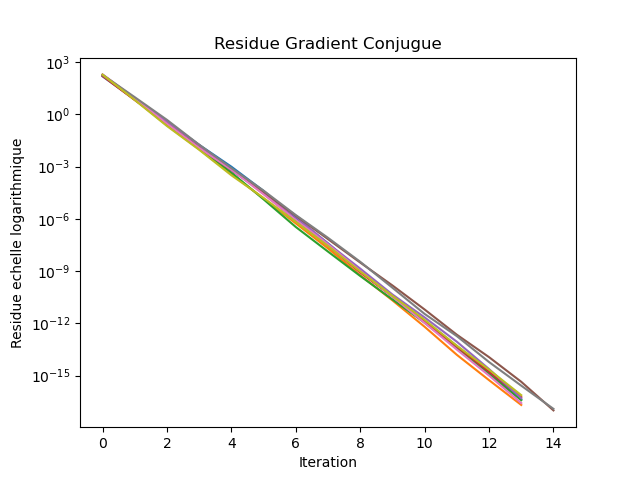
\includegraphics[width=\textwidth]{img/residue100.png}
    \caption{Évolution du résidu au fil des itérations pour 10 matrices de taille 100 (échelle logarithmique)}
    \label{fig:residue_100}
  \end{minipage}
  \hfill
  \begin{minipage}{0.55\textwidth}
    Contrairement à la méthode de Cholesky (section~\ref{sec:cholesky}), elle a une complexité linéaire par itération \(O(n)\).\\ \\
    \underline{\href{https://cours-mf.gitlabpages.inria.fr/is104/2-linear_systems/2-gc/}{L'implémentation proposée dans le sujet}} présente plusieurs problèmes, nous l'avons alors modifié pour inclure des vérifications, des noms de variables explicites, une condition d'arrêt flexible, et une meilleure gestion de la mémoire.\\ \\
    La figure~\ref{fig:residue_100} montre la décroissance exponentielle du résidu au fil des itérations pour des matrices de taille 100. Un préconditionneur pourrait améliorer cette méthode, mais n'a pas été implémenté ici.
  \end{minipage}
\end{figure}
De la même manière que pour la factorisation de Cholesky, nous avons comparé la précision des résultats obtenus pour notre implémentation méthode du gradient conjugué et celle de \texttt{scipy} avec la solution exacte. Pour cela, nous avons généré \(10 \times 496\) matrices aléatoires de taille \(n \times n\) avec \(n\) allant de 4 à 500. Nous avons ensuite moyenné l'erreur relative (selon la formule \(\frac{\| A \mathbf{x} - \mathbf{b} \|_1}{\| \mathbf{b} \|_1 \cdot n \cdot \epsilon}\)) et le temps d'exécution pour chaque taille de matrice.
\subsection{Application à l’équation de la chaleur}
L’équation de la chaleur en régime permanent est donnée par $\Delta T + f = 0$. En utilisant la formule de Taylor-Young et en travaillant dans un plan discret, on obtient $\frac{1}{h^2}AF=T$, où $A$ représente l'opérateur laplacien, et $F$ et $T$ sont des vecteurs de taille $N^2$, représentant respectivement le flux de chaleur et le champ de température.\\
Avant d'appliquer les deux méthodes, nous devons vérifier que $A$ est une matrice symétrique définie positive. On a $\forall i,j \in [1,N^2]$, $a_{(i,i-N)}=a_{(i-N,i)}=1$ (si $i>N$) et $a_{(i,i+N)}=a_{(i+N,i)}=1$ (si $i \leq N^2-N$), sinon $a_{(i,j)}=a_{(j,i)}=0$ ($i \neq j$). Ainsi, $A$ est bien une matrice symétrique.\\
De plus, $\forall i \in [1,N^2]$, $|a_{i,i}|=4$ et $\sum_{j \neq i} |a_{i,j}| \leq 4$, donc $A$ est une matrice à coefficients dominants et à diagonale positive. Par conséquent, d'après le théorème~\ref{thm:diag_dominant}, $A$ est une matrice symétrique positive.\\
Pour résoudre l'équation de la chaleur en régime stationnaire, nous devons résoudre le système linéaire $A\bar{T}=\bar{F}$ avec $\bar{F}=h²F$.
Il s'agit de résoudre le système $LL^T\bar{T}=\bar{F}$, soit $L\bar{Y}=\bar{F}$ puis $L^T\bar{T}=\bar{Y}$.
On a A possede $5N²-N-2$ coefficients non nuls et comme $\frac{5N^2-N-2}{N^4}$ est strictement décroissant et pour $N=10$ elle prend $0.0488$, donc le nombre des coefficients zéros à partir de $N=10$ est supérieur à $95.12\%$, donc c'est une matrice creuse.
\label{AN}
\section{Résultats et discussions}
Nous avons comparé les résultats obtenus pour la factorisation de Cholesky (complète et incomplète) et la méthode du gradient conjugué avec ceux de la bibliothèque \texttt{numpy} et la solution exacte.
\subsection{Décomposition de Cholesky}
Les résultats présentés figure~\ref{fig:cholesky} montrent que notre implémentation de la factorisation de Cholesky est plus précise que celle de \texttt{numpy}, probablement parce que \texttt{numpy} privilégie la performance.
\begin{figure}[H]
  \begin{minipage}{0.6\textwidth}
    \centering
    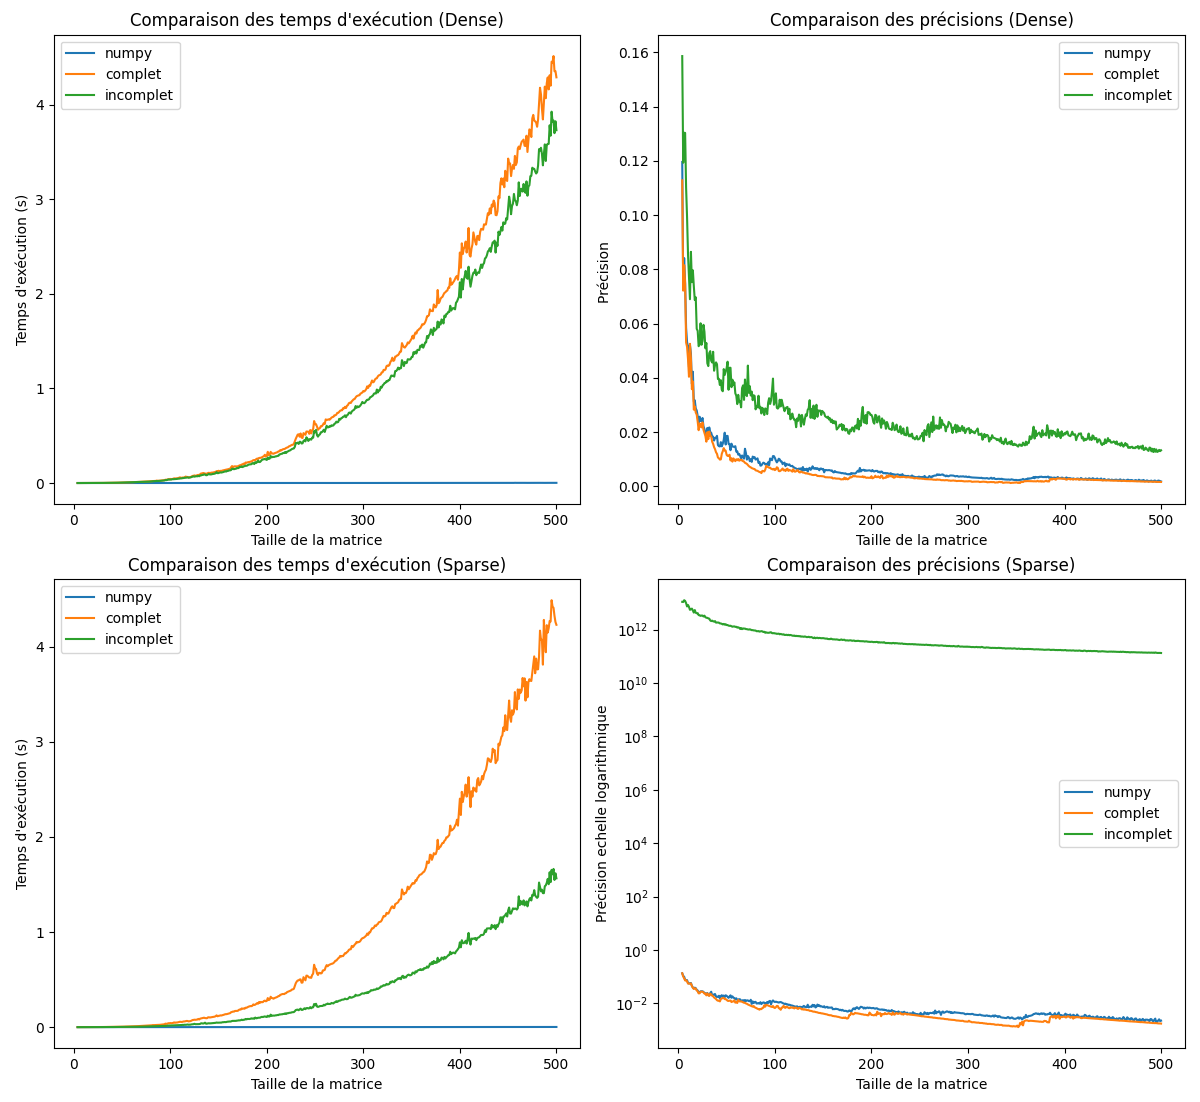
\includegraphics[width=\textwidth]{img/cholesky_all.png}
    \caption{Comparaison des résultats pour la factorisation de Cholesky pour des matrices denses et creuses}
    \label{fig:cholesky}
  \end{minipage}
  \hfill
  \begin{minipage}{0.35\textwidth}
     En termes de temps, la méthode complète est légèrement plus lente, mais la différence est négligeable pour des matrices de taille 100. Pour les matrices creuses, la précision est meilleure pour tous les algorithmes, mais la version incomplète de Cholesky est moins précise en raison de la perte d'information. \\
    La précision de \texttt{numpy} est similaire à celle de notre version dense. La précision de tous les algorithmes est relativement faible et décroît avec la taille de la matrice (erreur relative de l'ordre de \(10^{-2}\)). La version incomplète de Cholesky est avantageuse pour les matrices creuses car elle réduit la complexité de la factorisation et de la résolution des systèmes linéaires, malgré une précision moindre.
  \end{minipage}
\end{figure}
\subsection{Méthode du gradient conjugué }
Les résultats obtenus pour la méthode du gradient conjugué présentés figure~\ref{fig:gradient_conjugue} permettent d'observer que notre implémentation de la méthode du gradient conjugué est plus précise que celle de la bibliothèque \texttt{scipy}. Pour des raisons potentiellement similaires à celles évoquées pour la factorisation de Cholesky, la bibliothèque \texttt{scipy} pourrait privilégier la performance sur la précision.
\begin{figure}[h!]
  \begin{minipage}{0.5\textwidth}
    \centering
    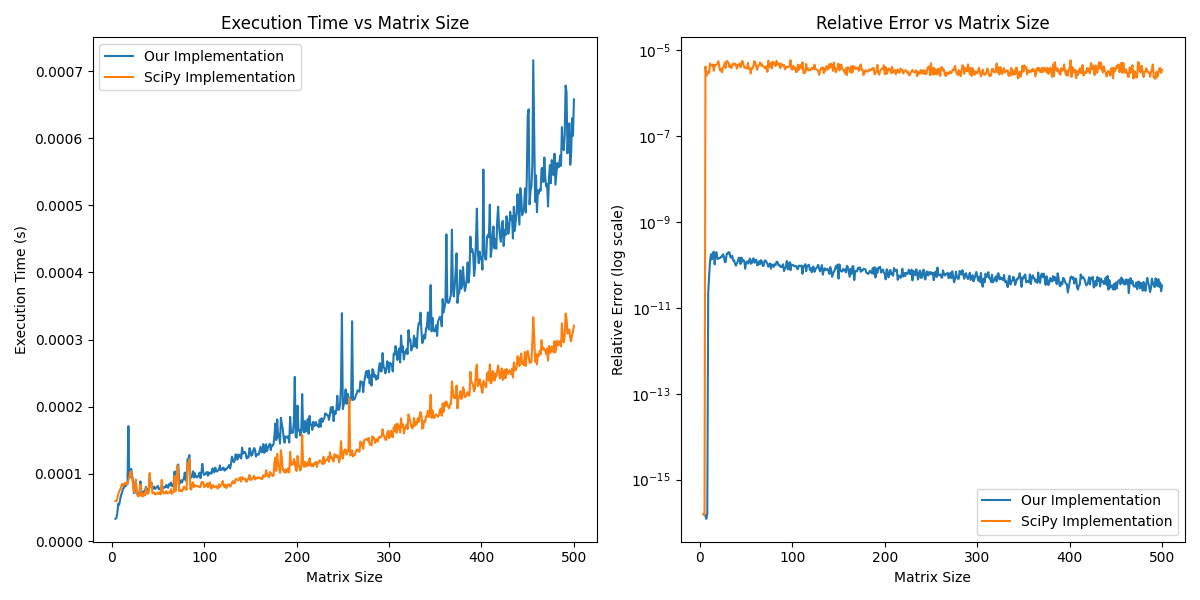
\includegraphics[width=\textwidth]{img/gradient_all.png}
    \caption{Comparaison des résultats pour la méthode du gradient entre notre implémentation et \texttt{scipy}}
    \label{fig:gradient_conjugue}
  \end{minipage}
  \hfill
  \begin{minipage}{0.45\textwidth}
    En termes de temps, la méthode du gradient conjugué est plus rapide que la méthode de Cholesky bien que notre implémentation soit moins performante que celle de \texttt{scipy}. \\
    La précision de la méthode du gradient conjugué est relativement faible et stable indépendamment de la taille de la matrice. La précision de \texttt{scipy} est quasiment similaire à celle de notre version.
  \end{minipage}
\end{figure}

\subsection{Application à l’équation de la chaleur}
En appliquant la méthode du gradient conjugué, et les deux factorisations de Cholesky, nous avons pu résoudre l'équation de la chaleur en régime stationnaire. Les résultats obtenus figure~\ref{fig:all_methods} montrent que l'ensemble des méthodes donnent des résultats similaires à l'exception de la méthode de Cholesky incomplète qui présente des erreurs plus importantes.

\begin{figure}[h!]
  \begin{center}
    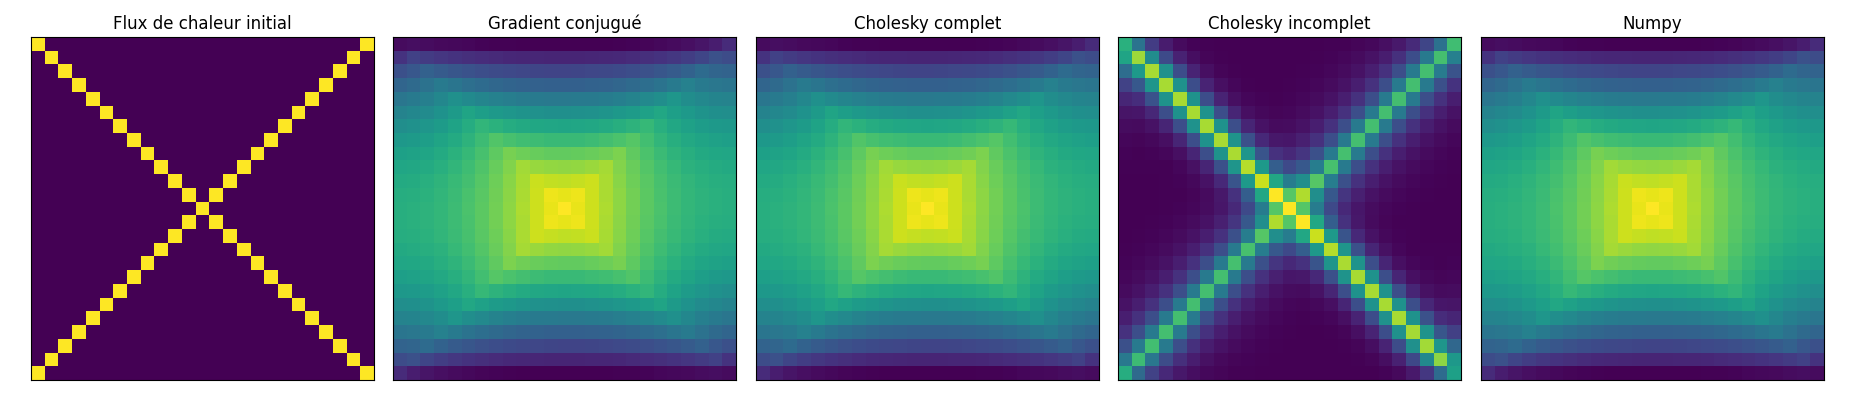
\includegraphics[width=0.6\textwidth]{img/compare_vis.png}
    \caption{Comparaison de la diffusion de la chaleur en croix sur une grille de taille \(25 \times 25\) avec une source de chaleur ponctuelle entre les différentes méthodes}
    \label{fig:all_methods}
  \end{center}
  \vspace{-1cm}
\end{figure}
\subsubsection{Cholesky}
\begin{multicols}{2}
  Sur la figure \ref{fig:all_methods}, on observe que la méthode complète donne de bons résultats, similaires à numpy. Cependant, Cholesky incomplet entraîne des erreurs et des écarts qui varient entre 0 et 7 (visible en figure~\ref{fig:chaleur}). Cela est dû au fait que, dans Cholesky incomplet, on ignore le calcul des coefficients correspondant au couple (i,j) tel que A[i][j]=0, ce qui entraîne des erreurs représentées en figure~\ref{fig:err_ch} qui montre la différence absolue entre A et LtL.
  \begin{figure}[H]
    \begin{center}
      \adjustbox{trim=0 0 0 0,clip}{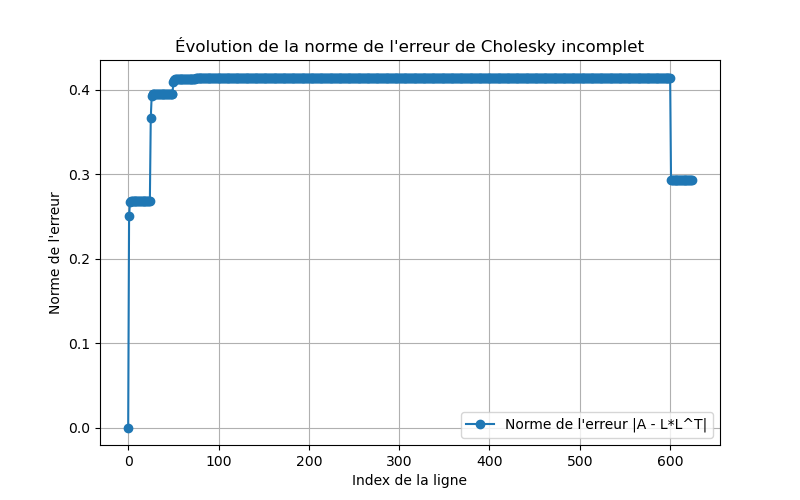
\includegraphics[width=0.4\textwidth]{img/erreur_cholesky.png}}
      \caption{Un exemple de la différence absolue entre A et LtL par Cholesky incomplet}
      \label{fig:err_ch}
    \end{center}
  \end{figure}
\end{multicols}
\subsubsection{Gradient conjugué}
\begin{figure}[H]
  \begin{minipage}{0.5\textwidth}
    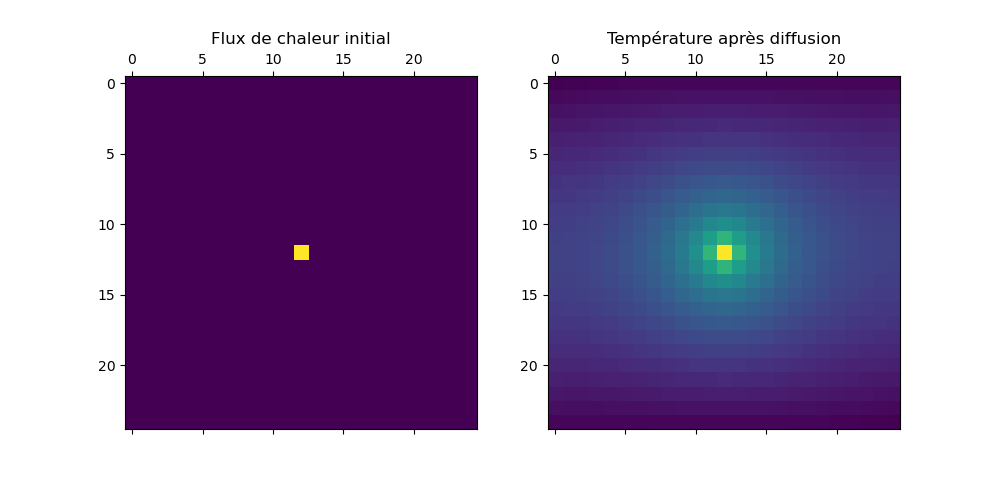
\includegraphics[width=\textwidth]{img/diff_1src.png}
    \caption{Diffusion de la chaleur avec une source de chaleur ponctuelle sur une grille de taille \(25 \times 25\), avant et après itérations}
    \label{fig:diff_1src}
  \end{minipage}
  \hfill
  \begin{minipage}{0.45\textwidth}
    En appliquant la méthode du gradient conjugué, nous avons pu résoudre l'équation de la chaleur en régime stationnaire. La figure~\ref{fig:diff_1src} montre la diffusion de la chaleur avec une source de chaleur ponctuelle. Nous observons que la température \(T\) représente bien la diffusion de la chaleur provenant de la source.\\
    Grâce à la méthode itérative du gradient conjugué, nous pouvons garder une trace de toutes les étapes intermédiaires, ainsi la figure~\ref{fig:diff_1src_evole} montre l'évolution de la diffusion de la chaleur pour une source en croix. 
  \end{minipage}
\end{figure}

\begin{figure}[H]
  \begin{minipage}{0.5\textwidth}
    Nous avons remarqué dans la section \ref{DEC_EXP} que le résidu décroît de manière exponentielle, ce qui implique que nous convergons rapidement vers la solution. Nous n'avons de ce fait pas présenté les 40 dernières itérations car la différence n'est plus visible à l'œil nu.\\
    Nous observons aussi que le nombre d'itérations est drastiquement inférieur à celui attendu théoriquement en effet nous avons 80 itérations au total au lieu de \(25 \times 25\) soit 625 attendues en théorie, cela peut s'expliquer par le fait que la matrice A est très creuse.
  \end{minipage}
  \hfill
  \begin{minipage}{0.45\textwidth}
    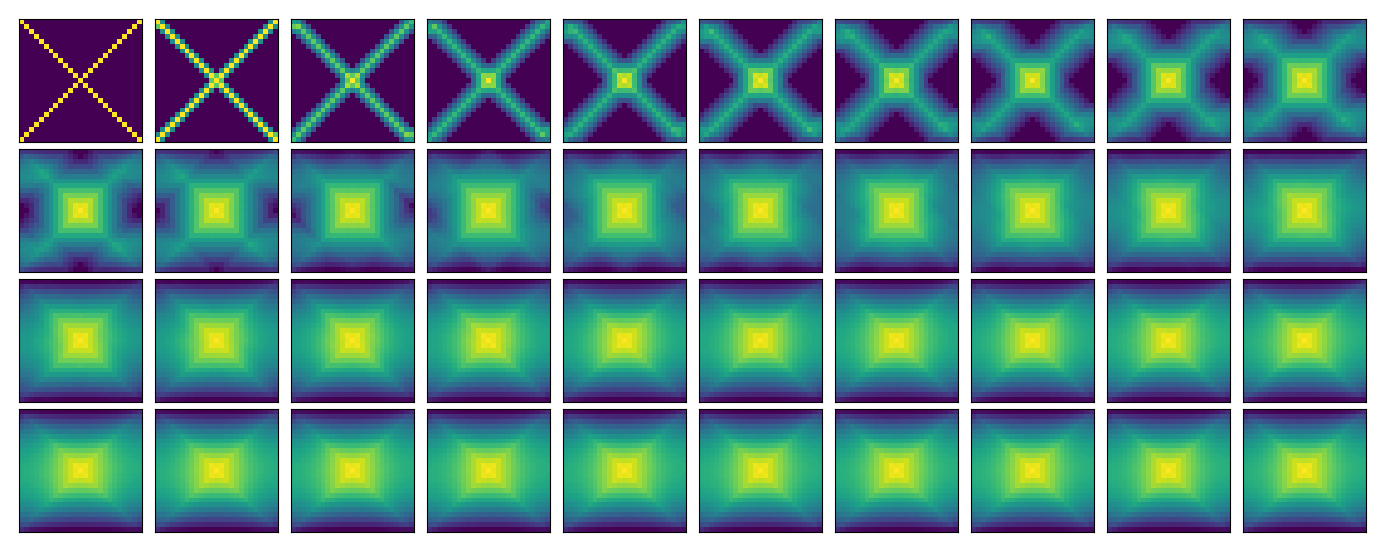
\includegraphics[width=\textwidth]{img/croixevol.png}
    \caption{Évolution de la diffusion de la chaleur avec une source de chaleur en croix}
    \label{fig:diff_1src_evole}
    
  \end{minipage}
\end{figure}


\subsubsection{Comparaison des méthodes}
\begin{figure}[H]
  \begin{minipage}{0.3\textwidth}
      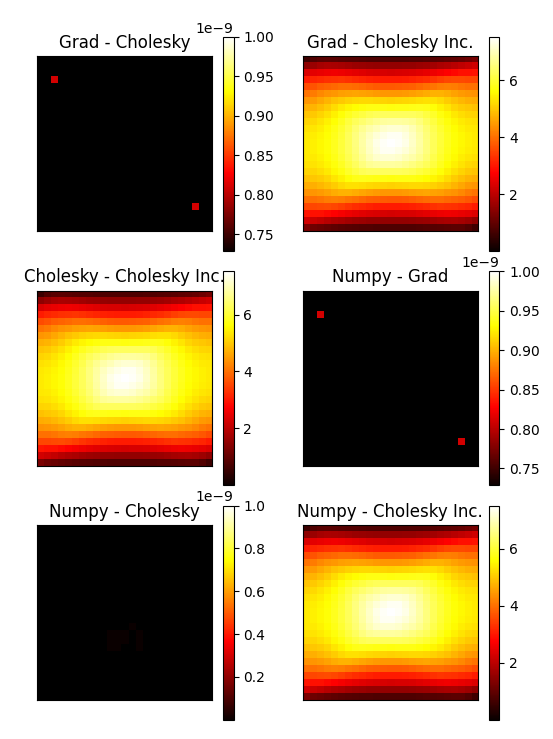
\includegraphics[width=\textwidth]{img/chaleur.png}
      \caption{Différences de pixels entre les méthodes pour la diffusion de la chaleur en croix (couleur claire = grande différence), échelle logarithmique}
      \label{fig:chaleur}
  \end{minipage}
  \hfill
  \begin{minipage}{0.65\textwidth}
    Pour mieux comparer les méthodes, la figure~\ref{fig:chaleur} montre les pixels divergents entre les différentes méthodes pour la diffusion de la chaleur en croix. Nous observons que la méthode du gradient conjugué donne des résultats similaires à la méthode de Cholesky complète et à \texttt{numpy}. Cependant, la méthode de Cholesky incomplète présente des erreurs plus importantes. La méthode du gradient conjugué est cependant moins précise à quelques pixels près, mais reste très proche de la solution exacte.
    \begin{figure}[H]
      \begin{center}
        \adjustbox{trim=0 5.5cm 0 1cm,clip}{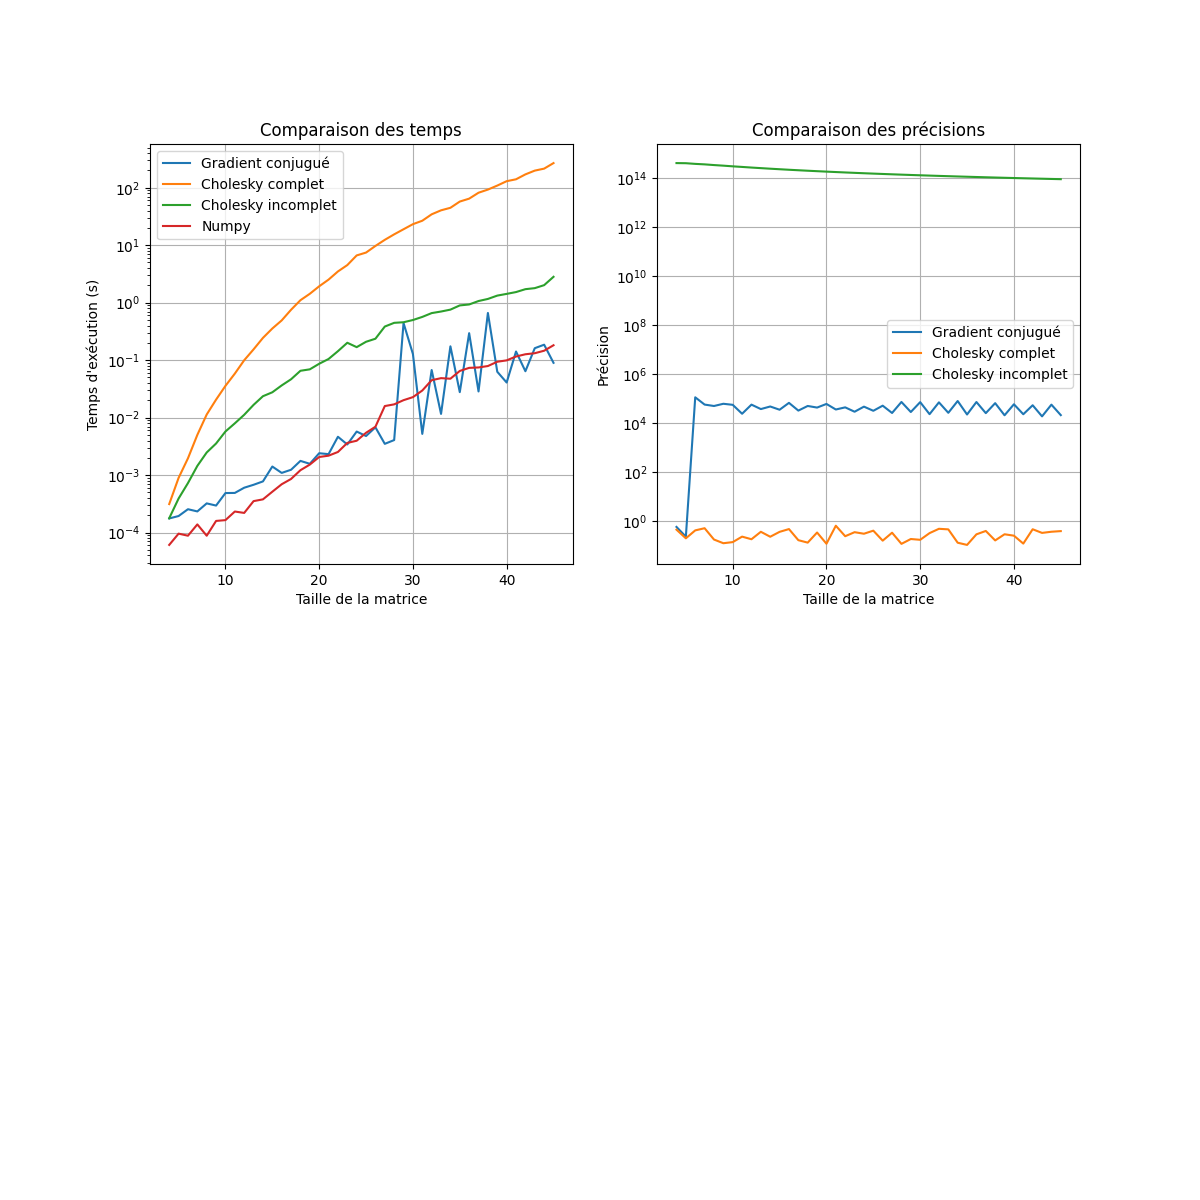
\includegraphics[width=\textwidth]{img/temps.png}}
        \caption{Comparaison des temps d'exécution et des erreurs relatives (par rapport à numpy) pour les différentes méthodes, échelle logarithmique.}
        \label{fig:comparaion_chaleur}
      \end{center}
    \end{figure}
  \end{minipage}
\end{figure}

Pour appuyer cette observation, la figure~\ref{fig:comparaion_chaleur} nous montre bien que la méthode du gradient conjugué est plus rapide que la méthode de Cholesky, mais moins précise. Et que la méthode de Cholesky très proche des résultats de numpy, malgré sa vitesse moindre. Compensée par sa version incomplète elle est néanmoins beaucoup moins précise.

\section{Conclusion et perspectives}
En conclusion, nous avons implémenté deux méthodes de résolution de systèmes linéaires, la décomposition de Cholesky et la méthode du gradient conjugué. Nous avons appliqué ces méthodes à la résolution de l'équation de la chaleur en régime stationnaire. Nous avons comparé les résultats obtenus pour toutes ces méthodes, ainsi qu'avec la bibliothèque \texttt{numpy}. Ce qui nous permet de conclure que la méthode du gradient conjugué pourrait représenter le meilleur compromis entre précision et performance pour la résolution de systèmes linéaires, bien que la méthode de Cholesky soit plus précise.\\
Pour aller plus loin, il serait intéressant d'implémenter un préconditionneur pour la méthode du gradient conjugué, ce qui permettrait de réduire le nombre d'itérations nécessaires pour converger vers la solution. Il serait également intéressant de tester ces méthodes sur des matrices de plus grande taille pour observer leur comportement.

\end{document}

